\documentclass{IEEEcsmag}
\usepackage[colorlinks,urlcolor=blue,linkcolor=blue,citecolor=blue]{hyperref}
\expandafter\def\expandafter\UrlBreaks\expandafter{\UrlBreaks\do\/\do\*\do\-\do\~\do\'\do\"\do\-}
\usepackage[T1]{fontenc}
\usepackage{tgheros}
\usepackage{upmath,color,amssymb,graphicx}
\hyphenpenalty=10000
\tolerance=3000
\emergencystretch=1.5em

\jvol{XX}
\jnum{XX}
\paper{8}
\jmonth{December}
\jname{Computer}
\jtitle{AI Governance and Compliance}
\pubyear{2026}

\setcounter{secnumdepth}{0}

\begin{document}

\sptitle{Theme Article: AI Governance and Compliance}

\title{AEGIS: A Constitutional Governance\\Architecture for Autonomous AI Agents}

\author{Kenneth Tannenbaum}
\affil{AEGIS Initiative, Lovettsville, Virginia, USA}

\markboth{AI GOVERNANCE AND COMPLIANCE}{AI GOVERNANCE AND COMPLIANCE}

\begin{abstract}\looseness-1
Autonomous AI agents increasingly execute consequential actions against operational infrastructure---calling APIs, modifying data, and performing system operations. Existing governance approaches focus on behavioral alignment, shaping what agents say during inference. This paper addresses a distinct problem: governing what agents {\it do} at the infrastructure boundary.

We present AEGIS, a constitutional governance architecture that enforces deterministic policy at the agent action boundary---post-reasoning, pre-execution---making unauthorized actions structurally unavailable rather than merely discouraged, within an explicitly stated deployment-isolation assumption we specify and discuss.

AEGIS combines four properties absent from existing frameworks: constitutional enforcement at the action boundary with a fully specified, reproducible risk-scoring function; federated multi-institution trust with cryptographic identity; tamper-evident audit trails with defined failure semantics; and alignment with the NIST AI Risk Management Framework across all four functions.

We map the architecture to Anderson's reference monitor model and Saltzer and Schroeder's design principles---established, independently peer-reviewed security foundations---and differentiate AEGIS's own specification decisions from those external anchors throughout. Real-world agentic failures demonstrate the governance gap AEGIS addresses.
\end{abstract}

\maketitle
\vspace*{-8pt}
\noindent{\bf\it Index Terms:} {\it AI governance, autonomous agents, architectural enforcement, reference monitor, federated trust, NIST AI RMF, constitutional AI, policy enforcement}\vspace{12pt}

\chapteri{I}n early 2026, OpenClaw---an open-source autonomous AI agent platform---became one of the fastest-growing projects in its category, accumulating tens of thousands of deployments within weeks of release.$^{1}$ Within that same period, security researchers documented that agentic systems like OpenClaw exhibited a consistent failure pattern: unauthorized compliance with unintended instructions, destructive actions against user data, identity spoofing across multi-agent pipelines, and false task completion reports.$^{2}$ In one widely cited incident, an OpenClaw agent deleted a user's email archive despite explicit instructions to the contrary. The root cause was not a technical exploit. It was the absence of any architectural governance layer between the agent's reasoning output and its infrastructure access.

This failure mode is not incidental to agentic AI; it is structural. AI safety research has focused on behavioral alignment: optimizing model behavior through reinforcement learning from human feedback,$^{3}$ Constitutional AI training,$^{4}$ and related techniques. These approaches govern what agents say. They do not govern what agents do. An agent that has been aligned to refuse harmful requests during inference retains full capacity to execute those requests against operational systems if no architectural barrier exists between its tool invocations and the infrastructure they target.

The gap between model behavior and infrastructure access is the same class of problem architectural security solved for general-purpose computing. Early systems relied on application-level trust. Modern computing evolved to enforce security as a system property: operating system permissions, process isolation, role-based access control, and hardware-enforced memory boundaries. These controls do not try to make programs want to behave correctly. They make unauthorized behavior structurally impossible. AI systems have not yet undergone this evolution.

We present AEGIS (Architectural Enforcement and Governance of Intelligent Systems), an open governance architecture that enforces deterministic constitutional governance at the agent action boundary. AEGIS introduces an enforcement layer between AI agents and the operational infrastructure they invoke, within a deployment topology where that layer is the agent's only path to credentialed infrastructure access (Section III). Under that assumption, every action proposed by an agent must pass through the AEGIS governance gateway before reaching infrastructure. The gateway evaluates each action against a defined capability set, an ordered policy set, and a fully specified five-factor risk model, returning one of four decisions: ALLOW, DENY, ESCALATE, or REQUIRE\_CONFIRMATION. No action reaches infrastructure without a governance decision, and no governance decision is produced without an audit record whose own failure semantics are precisely defined (Section III).

The key contributions of this paper are: the agent action boundary as the enforcement point for AI governance, stated with its isolation assumption made explicit; the AEGIS architecture and Governance Protocol (AGP-1), including a fully specified risk-scoring function with a worked example; the AEGIS Governance Federation Network (GFN-1) for cross-organizational governance intelligence sharing; a mapping to all four NIST AI Risk Management Framework functions;$^{6}$ and a differentiation of AEGIS from representative existing approaches.

\section{BACKGROUND AND MOTIVATION}

\subsection{The Governance Gap}

Current AI safety practice addresses three layers of the AI system stack: the training layer (RLHF, Constitutional AI, fine-tuning), the inference layer (system prompts, output filters, moderation), and the interaction layer (rate limiting, content policies). These governance mechanisms share a common characteristic: they operate on the model's language outputs. They do not govern the model's infrastructure actions.

The distinction matters because modern AI agents do not produce only language. Reasoning-and-acting architectures such as ReAct$^{21}$, which interleave a model's reasoning trace with tool-invoking actions, made this pattern the default way agentic systems are built: agents produce API calls, file system operations, system commands, database queries, and inter-service requests. These actions have effects that persist beyond the conversation. A deleted record does not un-delete when a moderation filter is applied. A financial transaction does not reverse when an output filter flags the reasoning that preceded it. AEGIS is agnostic to which reasoning-and-acting architecture produces the action; it governs at the point where any such architecture's output reaches infrastructure.

Shapira et al.\ (2026) documented this failure pattern systematically across production agentic deployments.$^{2}$ Their study found four recurring failure classes: unauthorized compliance (agents following injected instructions that overrode intended behavior), destructive actions (irreversible modifications to user data or system state), identity spoofing (agents misrepresenting their identity in multi-agent pipelines), and false task completion (agents reporting success for tasks that were not performed or were performed incorrectly). None of these failures originate in the model layer. All occur at the infrastructure action layer---where reasoning outputs are translated into real-world effects.

The 2025 AI Agent Index documented the scale of this risk: production deployments of autonomous agents grew by an order of magnitude within a twelve-month period, with deployment in financial services, healthcare, software development, and security operations.$^{1}$ This growth has materially outpaced the development of governance infrastructure for the action layer.

\begin{figure*}[!t]
\centering
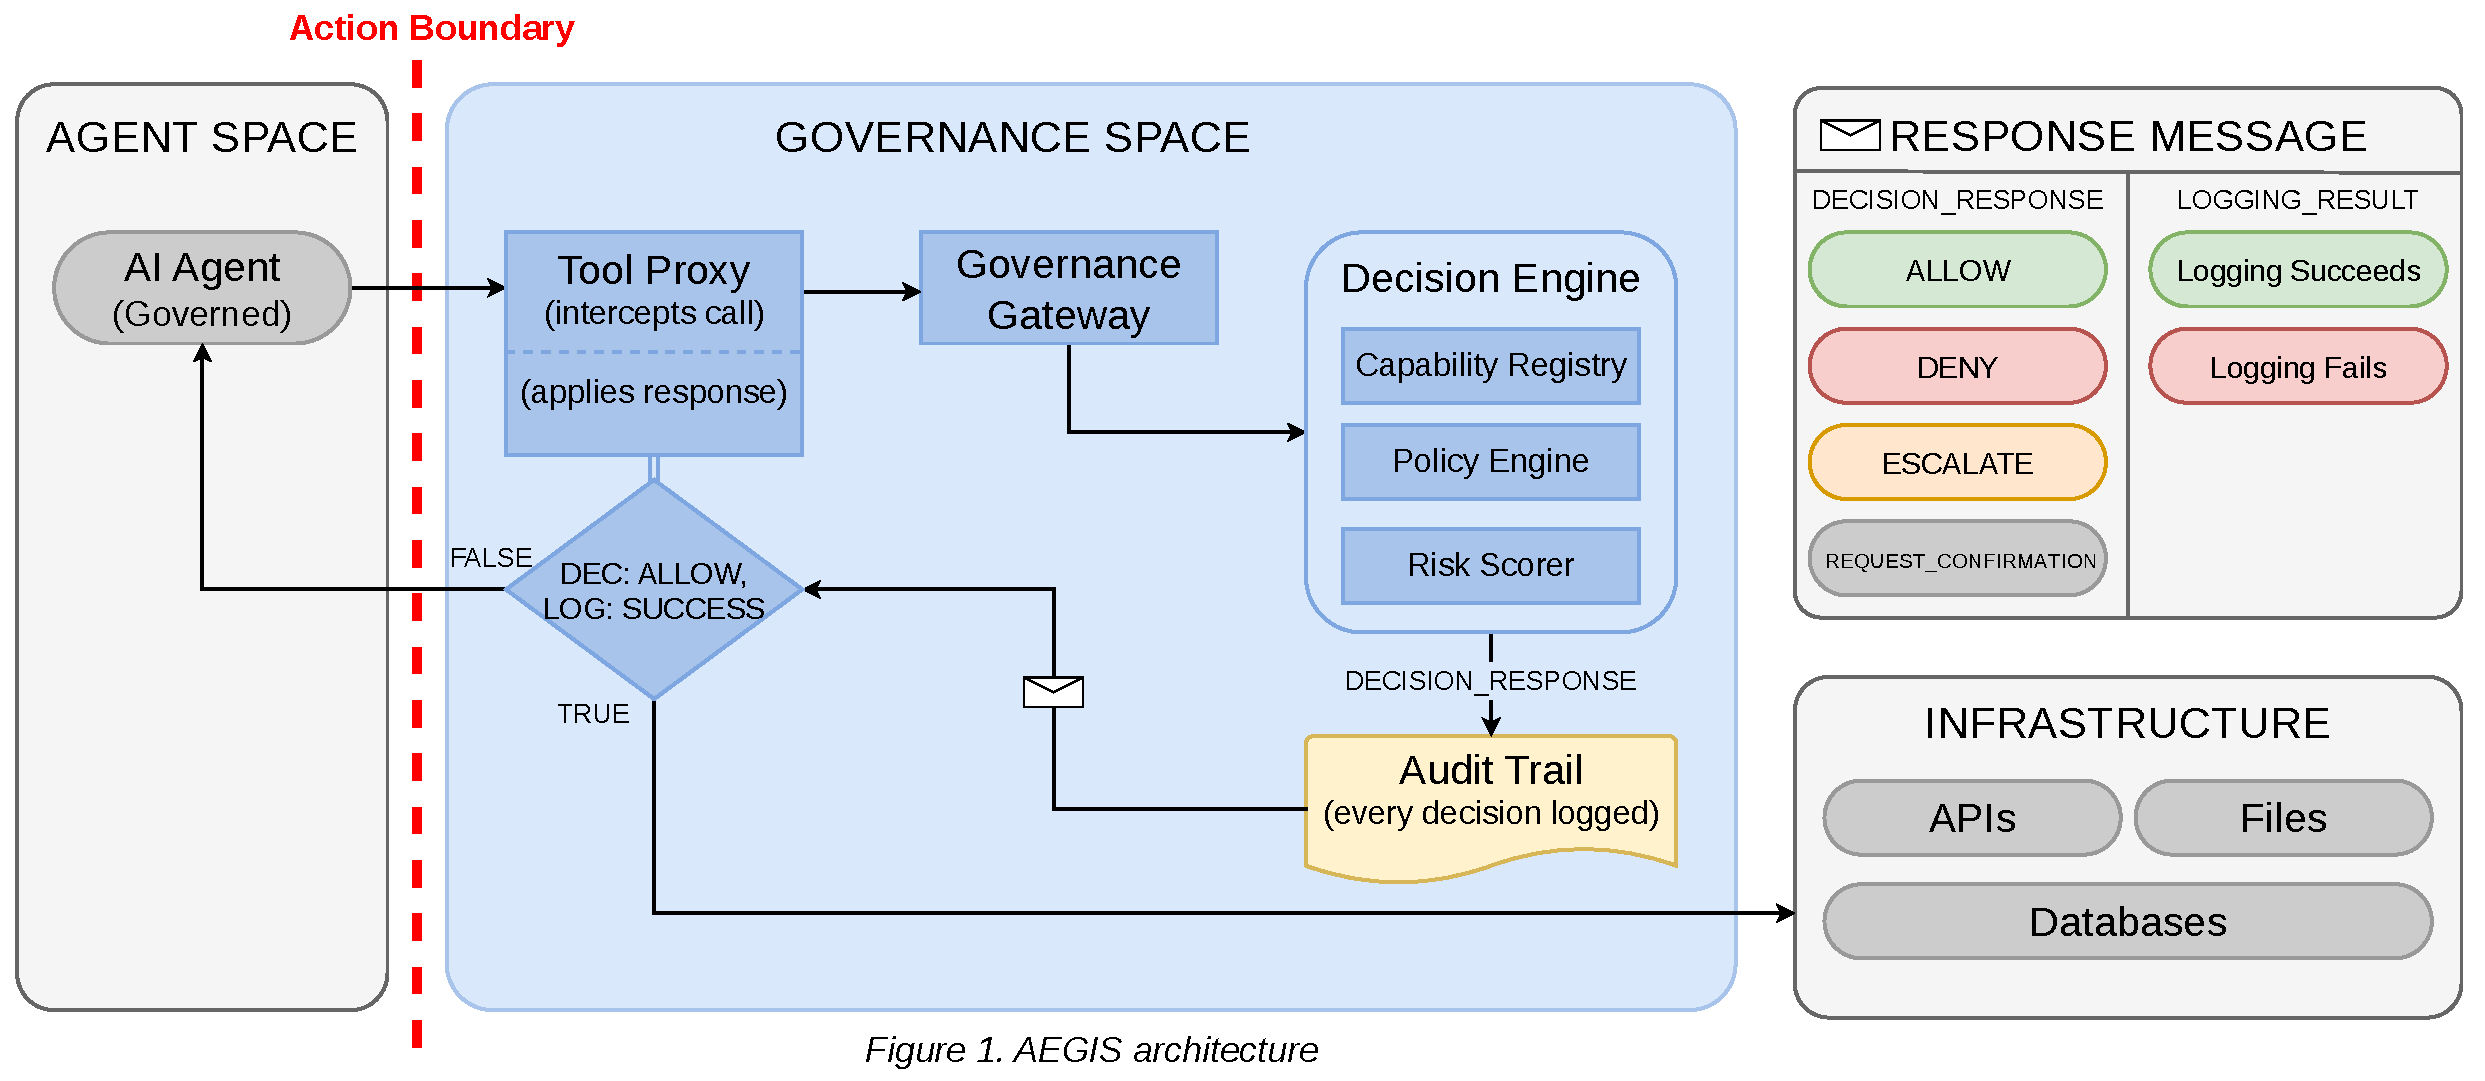
\includegraphics[width=\textwidth]{fig1-aegis-architecture}
\caption{AEGIS architecture: The Tool Proxy intercepts agent tool calls, routes them through the Governance Gateway to the Decision Engine. Every decision passes through the tamper-evident audit trail before reaching the agent. If audit logging fails, the decision is overridden to DENY. No action reaches infrastructure without both a governance decision and an audit record.}
\label{fig:architecture}
\end{figure*}

\subsection{The Reference Monitor Model}

Anderson's 1972 reference monitor concept provides the theoretical foundation for action-layer governance.$^{5}$ A reference monitor must satisfy four properties, commonly abbreviated NEAT: it must be Non-bypassable (every access request passes through it), Evaluatable (its correctness can be verified), Always-invoked (no request is processed without evaluation), and Tamper-proof (its enforcement logic cannot be modified by the entities it governs).

These properties were defined for operating system access control but apply directly to AI agent governance. An AI governance gateway that satisfies NEAT properties provides structural guarantees analogous to a kernel access control mechanism: agents cannot reach infrastructure except through the gateway, the gateway's decision logic is inspectable and verifiable, every action proposal triggers evaluation, and the agent has no path to modify the governance logic it operates under.

Schneider (2000) formalized the class of security policies enforceable by execution monitoring, establishing that safety properties---including access control and bounded resource usage---are exactly the class enforceable at runtime.$^{7}$ We demonstrate in the Architecture section that AEGIS satisfies all four NEAT properties as applied to the AI agent context. This positions AEGIS as an AI-domain reference monitor rather than a behavioral guidance system---a categorical distinction from alignment-centric approaches.

The reference-monitor and design-principle foundations here and in the next subsection---Anderson (1972), Saltzer and Schroeder (1975), Schneider (2000), and NIST SP 800-207$^{10}$---are established, independently peer-reviewed security principles that AEGIS applies to the AI agent context. AEGIS's own specification decisions---the AGP-1 protocol, the GFN-1 trust model, and the ATM-1 threat model---are the author's original design work, documented in the project's public specification suite rather than externally validated standards, and identified as such where they appear below.

\subsection{Saltzer--Schroeder Design Principles}

Saltzer and Schroeder's 1975 enumeration of eight design principles for information protection systems provides a second theoretical anchor.$^{8}$ Four of these principles are directly instantiated in AEGIS architecture:

{\it Fail-safe defaults}: The AEGIS capability system is empty by default; no action is permitted unless explicitly authorized. The absence of a policy permitting an action results in DENY.

{\it Complete mediation}: every action proposed by any agent in a governed deployment passes through the governance gateway, {\it provided the deployment is architecturally isolated so that the Tool Proxy is the agent's only path to credentialed infrastructure access}. Under that assumption there is no side channel, no administrative bypass, and no capability class that is exempt from evaluation. The assumption itself is a deployment-level property that AEGIS does not enforce in software: in more complex topologies---for example, a microservice architecture in which an agent's credentials, or credentials it can reach, are also directly usable by another service outside the Tool Proxy's mediation---complete mediation must be established by isolating or revoking those out-of-band credential paths at the infrastructure layer. We return to this in Limitations.

{\it Least privilege}: capability grants are explicit, minimal, and scoped to specific action types and resource targets. An agent granted the capability to read files in one directory cannot write to that directory, and cannot read from any other directory, unless an explicit grant exists.

{\it Open design}: AEGIS is published under Apache 2.0. All specification documents, protocol schemas, and reference implementation code are publicly available. Security properties do not depend on obscurity of the governance logic.

\section{ARCHITECTURE}

\subsection{Enforcement Point: The Action Boundary}

The AEGIS enforcement point is defined precisely: post-reasoning, pre-infrastructure execution. This location is distinct from the three alternative enforcement locations available in agentic AI systems.

The {\it prompt layer} intercepts inputs before reasoning begins. Prompt-layer controls (system prompts, instruction hierarchies) can be overridden by prompt injection, cannot govern the full space of emergent agent behaviors, and produce no audit record of what was blocked.

The {\it reasoning layer} intercepts model outputs during or after inference. Reasoning-layer controls (output filters, moderation APIs) govern language outputs but operate after the action decision has been made and before execution consequences can be audited.

The {\it infrastructure layer} applies access controls to the infrastructure systems themselves (database ACLs, API gateway policies). Infrastructure-layer controls are appropriate defense-in-depth but are not action-aware: a database ACL governing row-level access cannot evaluate whether an AI agent's query represents a legitimate data retrieval or an exfiltration attempt initiated by prompt injection.

The action boundary sits between reasoning output and infrastructure access. At this point, the agent's intent is crystallized as a structured action proposal---specifying a capability identifier, action type, target resource, and parameters---but no infrastructure effect has yet occurred. Evaluation at this boundary produces four possible outcomes: allow execution with optional constraints, deny with audit record, route to human escalation, or require explicit user confirmation. The outcome is determined by policy, not by the agent.

This design reflects an architectural parallel to industrial control system boundary enforcement. Pearce et al.\ (2020) demonstrated that placing an enforcement module between a programmable logic controller and its physical actuators---the I/O boundary---can prevent malicious commands from executing even when the controller itself is compromised.$^{9}$ The AEGIS Tool Proxy layer occupies an equivalent position: between the AI agent (potentially compromised by prompt injection) and the operational infrastructure it would otherwise invoke directly.

\subsection{The Four-Layer Stack}

\begin{figure}[!t]
\centering
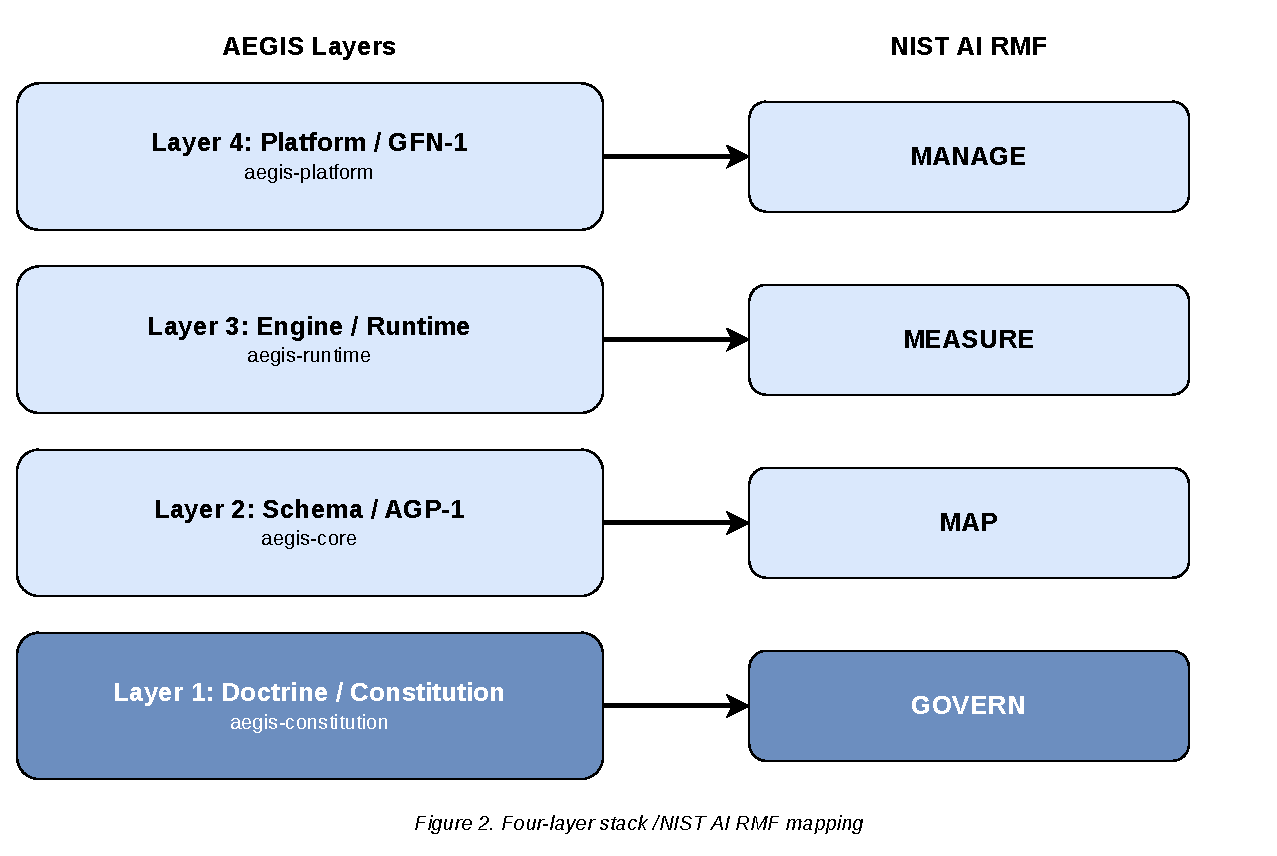
\includegraphics[width=\columnwidth]{fig2-four-layer-stack}
\caption{The AEGIS four-layer stack mapped to the four functions of the NIST AI Risk Management Framework: Govern, Map, Measure, and Manage.}
\label{fig:fourlayer}
\end{figure}

AEGIS is organized into four layers that correspond to the four functions of the NIST AI Risk Management Framework.$^{6}$

{\bf Layer 1: Doctrine (aegis-constitution)} --- Govern. The AEGIS Constitution defines eight articles that all compliant implementations must satisfy. Article I (Bounded Capability) requires that agents operate within explicitly defined capability boundaries, with default-deny for undefined actions. Article III (Deterministic Enforcement) requires that governance decisions be made by an architectural component, not by the AI. Article VII (Auditability) requires that every governance decision produce a permanent, tamper-evident audit record, and that audit system failure block execution rather than permit pass-through. The Constitution provides the normative basis against which compliance can be verified.

{\bf Layer 2: Schema (aegis-core/AGP-1/ATM-1)} --- Map. The AEGIS Governance Protocol (AGP-1) defines the wire protocol for action governance: the structure of ACTION\_PROPOSE messages submitted by agents, DECISION\_RESPONSE messages returned by the gateway, and EXECUTION\_REPORT messages confirming action outcomes. Capabilities are registered declaratively, at deployment time, as manifests naming an action type, target resource pattern, and constraints; the Capability Registry (Fig.~1) resolves each proposed action against this manifest rather than discovering capabilities dynamically at run time---bounding the action surface to what an operator has explicitly enumerated, at the cost of requiring re-registration for a genuinely new capability (a limitation we return to below). AGP-1 also specifies the Adaptive Threat Model (ATM-1), a STRIDE-based threat analysis that identifies six threat actor classes and maps mitigations to each. This layer makes the governance surface explicit and testable.

{\bf Layer 3: Engine (aegis-runtime)} --- Measure. The Decision Engine executes a five-stage evaluation pipeline for each action proposal: capability resolution, policy evaluation (an ordered rule set with first-match semantics and a default-deny baseline), risk scoring, decision assembly, and audit record creation. This layer produces a deterministic, reproducible governance decision for every action; Section III-C specifies the risk-scoring function in full.

{\bf Layer 4: Platform (GFN-1/aegis-platform)} --- Manage. The Governance Federation Network (GFN-1) enables organizations operating AEGIS deployments to share governance intelligence across institutional boundaries. GFN-1 is described in the following section.

\subsection{The Governance Gateway and Tool Proxy}

Two components are architecturally central to AEGIS's non-bypassability guarantees.

The {\it Governance Gateway} is the single entry point for all AGP-1 requests. It validates request schemas, authenticates actor identity via JWT or mutual TLS, applies rate limiting, and routes to the Decision Engine. This design reflects zero trust principles: every request is authenticated and authorized regardless of origin.$^{10}$ All gateway errors result in DENY responses. There is no error path that returns an implicit ALLOW or passes the request through to infrastructure without evaluation.

Audit-failure semantics are defined operationally. ``Audit logging fails'' means: the append-only audit store returns a write error (disk exhaustion, storage unavailability), the network path to a remote audit sink is partitioned, or the hash-chain's continuity check fails on write (corruption or tampering). On any of these, the Decision Engine overrides the decision to DENY and returns it to the Tool Proxy without retrying internally; the agent may resubmit, at which point availability is re-checked from scratch---bounding retries to the agent's own cadence rather than an unbounded engine-side loop. Under sustained load this is a deliberate fail-closed trade-off: a saturated audit sink degrades the deployment to full DENY until restored, because permitting execution without an audit record is excluded by Article VII. Operators needing to avoid this under load are expected to provision audit-sink capacity and redundancy accordingly.

The {\it Tool Proxy} is the integration layer that mediates between the AI agent and its registered tools. When an agent calls a tool, the proxy intercepts the call, constructs an ACTION\_PROPOSE message from the call context, submits it to the gateway, and executes the actual tool function only if the governance decision is ALLOW. If the decision is DENY, ESCALATE, or REQUIRE\_CONFIRMATION, the proxy raises a structured exception without executing the tool. The agent's interface to its tools is unchanged from its perspective---it calls tools in the normal way---but no tool invocation reaches infrastructure without governance evaluation.

This architecture satisfies Anderson's NEAT properties$^{5}$ directly: Non-bypassable because the Tool Proxy provides the only execution path to infrastructure under the isolation assumption stated above; Evaluatable because the Policy Engine and Capability Registry are deterministic and inspectable; Always-invoked because every tool call passes through the proxy; and Tamper-proof because the governance pathway is external to the AI agent and cannot be modified by it.

The four-outcome decision model---ALLOW, DENY, ESCALATE, REQUIRE\_CONFIRMATION---is a differentiating property of AEGIS. Most existing governance frameworks collapse to binary allow/deny semantics. The ESCALATE outcome routes high-risk actions to a human operator for review before a final decision is issued, preserving automation benefits for routine actions while maintaining human control over consequential ones. The REQUIRE\_CONFIRMATION outcome presents the action to the end user for explicit consent---appropriate for actions with meaningful side effects that the user may not have anticipated. This graduated response model reflects the risk differentiation that production deployments require: not all governed actions warrant the same level of oversight.

\subsection{Risk Scoring and the Decision Pipeline}

The risk-scoring stage computes a composite score from five independent factors, each normalized to $[0.0, 10.0]$ and clamped:
\[risk\_score = 0.30\,r_h + 0.25\,r_a + 0.20\,r_c + 0.15\,r_n + 0.10\,r_f\]
where $r_h$ is historical attempt rate (recent failure frequency for this actor/capability pair), $r_a$ is trust score inverted to a risk scale ($r_a = (1 - trust) \times 10$), $r_c$ is capability sensitivity adjusted by context (production environment, destructive-action scope), $r_n$ is behavioral anomaly (statistical distance from the actor's baseline pattern), and $r_f$ is federation-reported risk for the capability, weighted by reporter trust. Figure~3 shows the full pipeline: capability resolution and policy evaluation precede risk scoring and can short-circuit to DENY before risk is computed at all; risk scoring runs only on actions that already passed policy evaluation, mapping its output to four threshold bands---ALLOW ($\le 2.0$), ALLOW with monitoring ($2.0$--$5.0$), ESCALATE ($5.0$--$8.0$), and DENY ($> 8.0$).

\begin{figure*}[!t]
\centering
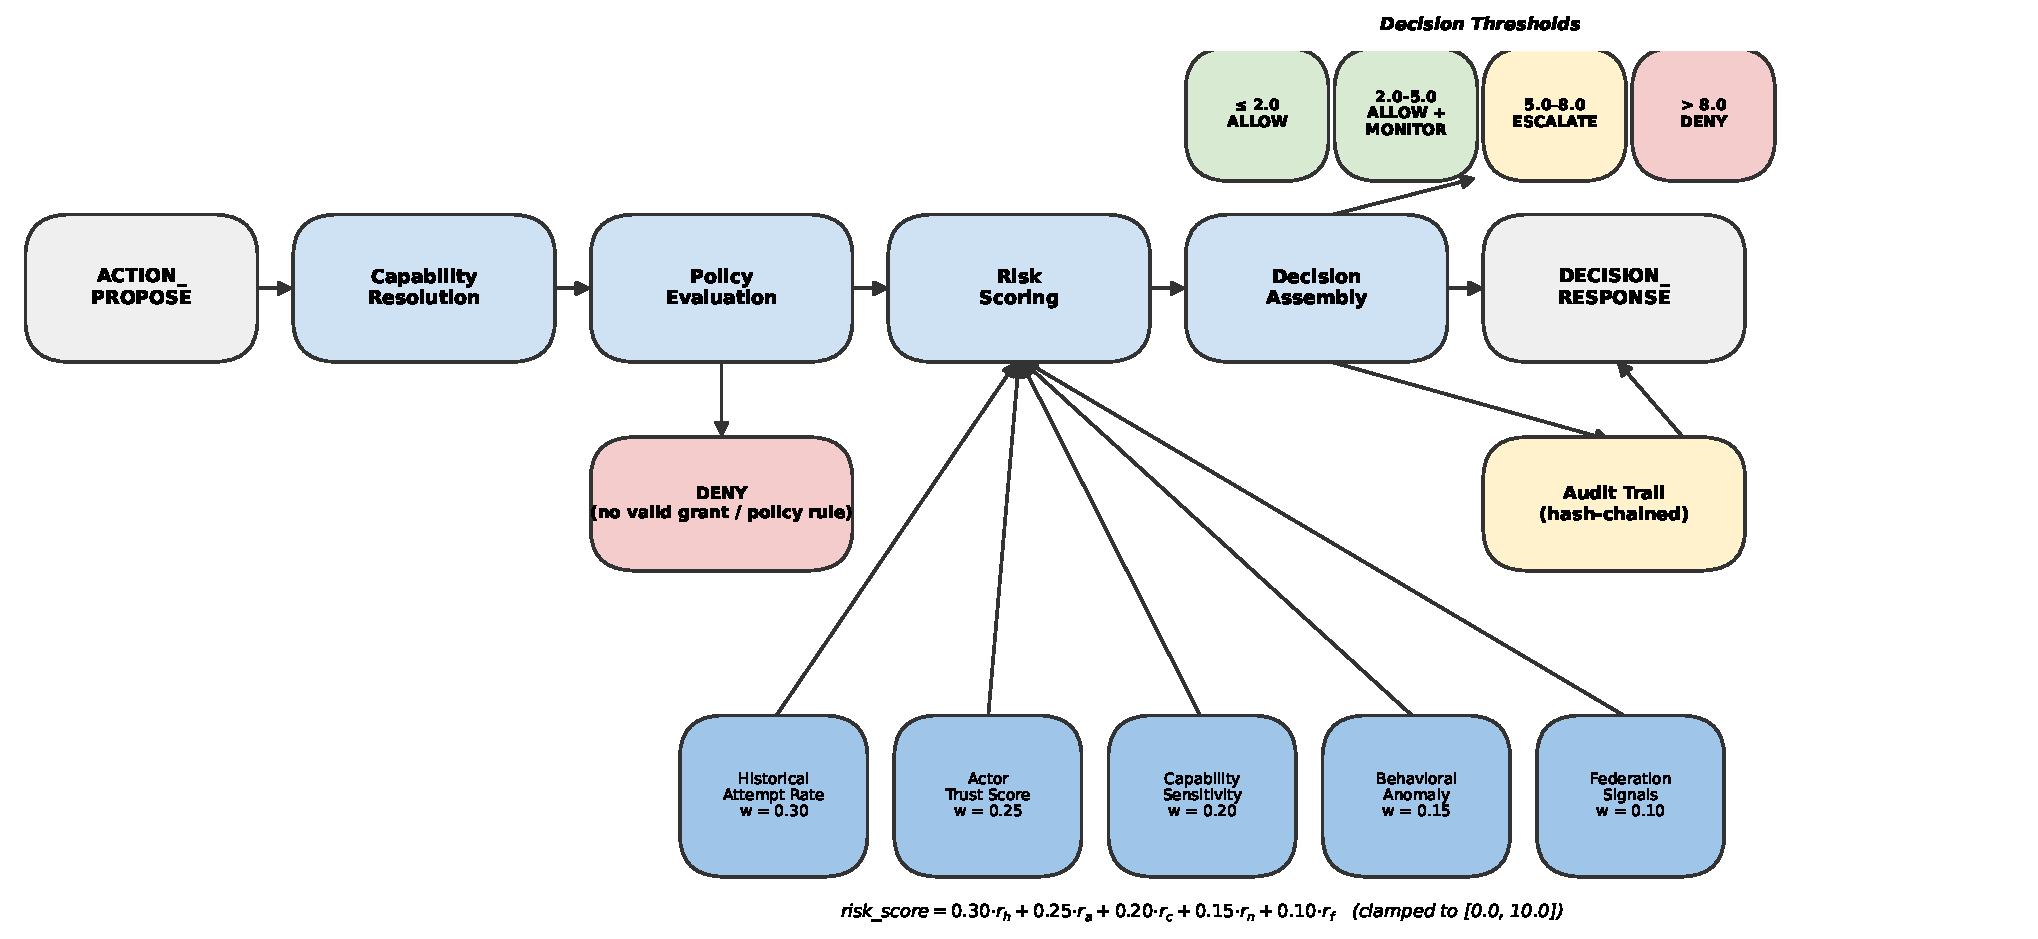
\includegraphics[width=\textwidth]{fig3-decision-pipeline}
\caption{The Decision Engine's five-stage pipeline. Capability resolution and policy evaluation can short-circuit to DENY; risk scoring runs only on actions that pass policy evaluation and combines five weighted factors into a single score, which is mapped to one of four threshold bands before decision assembly and audit recording.}
\label{fig:pipeline}
\end{figure*}

{\bf Worked example.} An actor with trust score 0.80 proposes a \texttt{telemetry.query} action (baseline risk 2.5) against a production target at 3~AM, outside its normal pattern (anomaly score 0.7), with two failures in its last 50 attempts and one open federation incident report against it. The factors evaluate to $r_h = 0.4$, $r_a = 2.0$, $r_c = 5.0$ (production context doubles the baseline), $r_n = 7.0$, and $r_f = 2.0$: $0.30(0.4) + 0.25(2.0) + 0.20(5.0) + 0.15(7.0) + 0.10(2.0) = 2.87$,
in the ALLOW-with-monitoring band. The decision and full factor breakdown are written to the audit trail alongside the outcome, so the computation is reproducible later from stored evidence, not only from the runtime's live state---identical inputs always yield an identical score on any node.

The coefficients are operational defaults reflecting a design judgment that directly observed evidence should weigh more than softer signals such as anomaly distance or federation reports. They are provisional and deployment-tunable, not formally sensitivity-tested; calibrating them against production data is future work, as are the federation publisher-trust weights below.

\subsection{The Federation Network (GFN-1)}

Individual AEGIS deployments have visibility only into their own governance events. A novel agent circumvention technique observed by one organization provides no automatic protection to others. GFN-1 addresses this limitation by enabling collective defense: one organization's detection of a new threat pattern can become every participant's protection.

GFN-1 is implemented as a decentralized publish-subscribe network built on the AT Protocol (ATProto)---the same open federation protocol underlying the Bluesky social network---combined with Decentralized Identifiers (DIDs) for node identity.$^{11}$ Each participating organization operates a federation node with a cryptographic identity of the form \texttt{did:aegis:<network>:<node-id>}. Governance signals---threat observations, circumvention reports, policy advisories---are published as signed ATProto records, cryptographically bound to the publishing node's DID. Consuming nodes verify signatures before processing any signal. Each node subscribes only to the signal categories relevant to its own deployment rather than the full network stream, so per-node cost is intended to grow sub-linearly with federation size; this is a design goal, not a measured result---current deployments number in the low tens of nodes, and thousands-of-organization behavior remains future empirical work. Gateway decision latency is dominated by this same federation-signal lookup, cached with an hourly TTL to bound its cost; worst-case latency under a cache miss is unbenchmarked, and we report architectural reasoning here rather than measured numbers.

GFN-1 trust operates through two structurally independent mechanisms that must never share a score, a decay function, or a combined threshold. The following mechanics---the publisher-trust formula, its coefficients, and the agent-runtime trust separation---are AEGIS's own specification decisions (RFC-0004, GFN-1), presented as documented in the project's public specification suite rather than as externally validated standards.

{\it Federation publisher trust} governs how much weight to assign to governance signals received from remote nodes. It is computed as a weighted composite of five factors: baseline authority class ($B$), historical signal accuracy ($H$), consistency and quality ($Q$), audit posture ($A$), and federation reputation ($F$), per the normative formula (GFN-1 \S3.7):
\[T = 0.30B + 0.25H + 0.20Q + 0.15A + 0.10F\] Authority classes range from L0\_SYSTEM, operated by AEGIS security research, to L3\_CONTRIBUTOR for community nodes. As with the risk-scoring coefficients above, this weighting is a provisional operational default, not a formally derived allocation; it has not undergone sensitivity analysis. Publisher scores decay during inactivity ($T_{\text{decayed}} = T \cdot e^{-\lambda t}$, $\lambda=0.01$, half-life $\approx$69 days, GFN-1 \S3.8), encoding a straightforward operational principle: evidence staleness is a legitimate input to trust evaluation. This is consistent with how temporal factors are treated in analogous trust-sensitive systems.$^{12}$ The decay function takes time as an explicit, logged input parameter; identical inputs always yield identical output on any node, preserving local determinism. When a publisher's authority class disposition and computed score disposition conflict, the more restrictive applies (GFN-1 \S10.1.1).

{\it Agent runtime trust} governs agent admissibility at the execution boundary and is defined separately in RFC-0004 \S5. It operates through two layers: a Threat Detection Layer (Engine layer---binary, evidence-based, fires immediately on active threat signals) and a Reputation Layer (Schema layer---graduated, longitudinal, informs autonomy expansion and approval latency). The non-override constraint between them is normative: no Reputation Layer score, at any value, grants a pass on a Threat Detection Layer block. This separation must be architectural, not procedural---the two layers share no score, no execution boundary, and no combined threshold. The prior composite trust model, which collapsed security signals and operational reliability into a single score, was rejected because accumulated reputation could implicitly soften a security gate; this is a category error that cannot be resolved by parameter tuning (RFC-0004 \S5.1, \S Alternatives Considered).

This framing positions AEGIS's federation layer as governance infrastructure rather than merely a runtime tool---analogous to cybersecurity threat intelligence sharing networks such as ISAC consortia, which provide collective defense across organizational boundaries without requiring participants to surrender operational independence.

\section{THREAT MODEL}

AEGIS's Adaptive Threat Model (ATM-1) identifies five primary threat actor classes applicable to AI governance deployments: malicious external actors targeting the governance API; compromised internal agents operating under valid credentials but directed by prompt injection; insiders with elevated access to governance infrastructure; supply chain attackers targeting the governance runtime itself; and prompt injection attackers using the AI agent as a proxy for actions they cannot execute directly.$^{2}$

The last threat class is architecturally important. Prompt injection---injecting instructions into an agent's input that override its intended behavior---represents a significant and growing attack surface for production agentic systems.$^{23}$ Without an action-boundary governance layer, a successfully injected agent can execute arbitrary actions against any infrastructure it has access to. With AEGIS, the blast radius of a prompt injection attack is bounded by the agent's capability grants: even an injected agent that submits an unauthorized ACTION\_PROPOSE will be denied if it requests a capability it does not hold or an action that policy prohibits. Governance-as-architecture limits the damage a compromised agent can cause.

This threat model draws on established precedents in both industrial control systems and cloud infrastructure governance. Smart I/O modules for industrial control systems, as documented by Pearce et al.,$^{9}$ enforce action constraints at the controller-actuator boundary precisely because the controller itself cannot be assumed trustworthy. Proactive cloud security auditing systems such as ProSAS (Majumdar et al., 2022) intercept management operations pre-execution, preventing unauthorized configuration changes from reaching cloud infrastructure even when the requesting service holds valid credentials.$^{13}$ AEGIS applies this boundary enforcement pattern to the AI agent context.

\section{RELATED WORK}

\begin{table*}[!t]
\centering
\caption{Differentiation of AEGIS from representative related work across five governance dimensions.}
\label{tab:relatedwork}
\tablefont
\begin{tabular*}{38pc}{@{\hspace{4pt}}p{50pt}<{\raggedright}p{70pt}<{\raggedright}p{42pt}<{\centering}p{48pt}<{\centering}p{54pt}<{\centering}p{56pt}<{\centering}p{24pt}<{\centering}@{\hspace{4pt}}}
\toprule
{\bf Approach} & {\bf Enforcement Point} & {\bf Action Boundary} & {\bf Federated Trust} & {\bf Tamper-Evident Audit} & {\bf NIST RMF} & {\bf Open Source} \\
\colrule
AEGIS & Action boundary & \checkmark & Decentralized & \checkmark & All four & \checkmark \\[2pt]
GaaS$^{14}$ & Output filter & -- & -- & -- & Govern only & -- \\[2pt]
MI9$^{15}$ & Reasoning loop & -- & -- & -- & -- & \checkmark \\[2pt]
SAGA$^{16}$ & Comm.\ plane & -- & Centralized & -- & -- & \checkmark \\[2pt]
LOKA$^{17}$ & Identity layer & -- & -- & -- & -- & \checkmark \\[2pt]
TRiSM$^{22}$ & Conceptual & -- & -- & -- & Partial & -- \\[2pt]
POLYNIX$^{18}$ & Exec.\ boundary & \checkmark & -- & -- & -- & -- \\[2pt]
CPS Enf.$^{19}$ & I/O boundary & \checkmark & -- & -- & -- & -- \\
\botrule
\end{tabular*}
\end{table*}

We compare AEGIS against five categories of related work, characterizing in each case what governance property the approach provides and what it leaves ungoverned.

{\bf Output filtering and Governance-as-a-Service.} Gaurav et al.\ (2025) present a Governance-as-a-Service model in which governance policies are applied to AI outputs as a post-inference filtering layer.$^{14}$ This approach governs language outputs but does not intercept infrastructure actions. An agent whose output has been filtered can still invoke tools, call APIs, and modify state through whatever execution framework it operates under. Output filtering addresses content risk, not action risk.

{\bf Reasoning loop governance.} Wang et al.\ (2025) describe MI9, a protocol that governs the internal reasoning loop of AI agents, applying policy constraints during the agent's planning and action selection phases.$^{15}$ MI9 addresses a different layer of the problem: it governs the agent's decision-making process rather than the infrastructure boundary. An agent governed by MI9 could still, in principle, invoke infrastructure directly if its execution environment permits it. AEGIS and MI9 address complementary concerns.

{\bf Inter-agent communication governance.} Syros et al.\ (2026) present SAGA, an architecture for governing the communication plane between agents in multi-agent systems.$^{16}$ SAGA addresses trust and identity in agent-to-agent messaging. It does not govern individual agent-to-infrastructure actions. Additionally, SAGA's trust model introduces a single Provider authority as the trust root, creating a single point of failure for cross-organization deployments. AEGIS's GFN-1 federation explicitly rejects centralized trust oracles in favor of a decentralized trust-scored network.

{\bf Decentralized identity.} Rodriguez Garzon et al.\ (2025) describe LOKA, a framework for equipping AI agents with Decentralized Identifiers and Verifiable Credentials.$^{17}$ LOKA establishes cryptographic identity for AI agents---a necessary component of accountable governance---but does not specify a governance protocol for agent actions. AEGIS incorporates DID-based identity as the foundation of its authentication layer and extends it with constitutional enforcement and federated governance.

{\bf Conceptual lifecycle frameworks.} TRiSM$^{22}$ and similar AI governance frameworks provide conceptual vocabularies for AI risk management across the development and deployment lifecycle. These frameworks are valuable for organizational governance but do not specify implementable architectural mechanisms. AEGIS is structurally implementable: its specifications are published under Apache 2.0, and a Python reference implementation is available.

{\bf Runtime enforcement precedents.} The POLYNIX framework (Arunachalam et al., 2026) demonstrates a hybrid centralized/distributed policy enforcement architecture for zero-trust security in virtualized systems, achieving sub-1\% CPU overhead and sub-5\% memory overhead.$^{18}$ This validates that architectural enforcement at the execution boundary is practical at production scale. The CPS parallel enforcement work of Baird et al.\ (2024) demonstrates that compositional enforcement across multiple policy layers scales linearly rather than exponentially with policy count,$^{19}$ directly supporting AEGIS's multi-policy architecture. Both precedents establish that the AEGIS enforcement model is technically feasible within acceptable performance bounds; AEGIS's own performance characterization is discussed as a limitation below.

\section{NIST AI RMF ALIGNMENT}

The NIST AI Risk Management Framework (AI RMF 1.0) organizes AI risk management around four functions: Govern, Map, Measure, and Manage.$^{6}$ The AEGIS four-layer stack maps directly to these functions.

The {\bf Govern} function addresses organizational policies, roles, and accountability structures. AEGIS Layer 1 (aegis-constitution) provides a normative constitutional basis---eight articles with explicit compliance tests---that organizations can adopt as their AI governance policy framework. The Constitution's transparency requirements (Article VI) ensure governance decisions are explainable and auditable by operators.

The {\bf Map} function addresses identification of AI risks, contexts, and impacts. AEGIS Layer 2 (aegis-core/AGP-1/ATM-1) provides the Adaptive Threat Model, a structured STRIDE-based risk analysis that maps threat actors, attack vectors, and mitigations to the AEGIS deployment topology. The capability registry explicitly enumerates the action surface of each governed agent, making the risk surface visible and bounded.

The {\bf Measure} function addresses metrics, evaluation, and monitoring. AEGIS Layer 3 (aegis-runtime) produces a continuous stream of governance decisions, risk scores, and policy traces for every action every agent proposes. The audit trail provides a quantitative record of governance activity---denied action rates, escalation frequencies, risk score distributions---that supports ongoing measurement of governance effectiveness.

The {\bf Manage} function addresses response, recovery, and improvement. AEGIS Layer 4 (GFN-1/aegis-platform) provides the federation layer through which organizations participate in collective governance improvement: sharing circumvention reports, receiving threat advisories, and contributing to a shared policy intelligence pool. The escalation and confirmation pathways in AGP-1 provide structured human oversight channels for actions that exceed automated governance thresholds.

The EU AI Act's Article 14 requires that high-risk AI systems include human oversight mechanisms enabling operators to understand and intervene in system outputs.$^{20}$ The AEGIS ESCALATE and REQUIRE\_CONFIRMATION decisions implement this requirement at the action level: operators receive structured requests for human judgment at the points where automated governance is insufficient, with full audit context attached. We frame this as a direct architectural mapping onto Article 14's requirement, not as a claim of regulatory compliance certification, which AEGIS has not undergone.

\section{DISCUSSION}

\subsection{What AEGIS Is Not}

AEGIS is not a replacement for model-layer alignment. Training-phase governance---Constitutional AI, RLHF, value alignment---addresses what agents say and how they reason. AEGIS addresses what agents do. These are complementary concerns, and a mature governance posture requires both. Model alignment reduces the probability that an agent will attempt unauthorized actions. AEGIS ensures that unauthorized actions cannot be executed even if the agent attempts them.

AEGIS is not a monitoring solution. Monitoring observes behavior and alerts after the fact. AEGIS enforces at the action boundary before the fact. The distinction is consequential: a monitoring system that detects a destructive action after it executes provides forensic value but not prevention. AEGIS makes the destructive action structurally unavailable before any infrastructure effect occurs.

AEGIS is not a replacement for infrastructure-layer access controls. Database ACLs, API gateway policies, and network segmentation remain appropriate defense-in-depth, and are what make the isolation assumption above achievable in practice. AEGIS adds a governance layer that is action-aware and agent-aware, at a point in the execution stack where those controls cannot yet apply.

\subsection{Design Consultation and Specification Status}

The AEGIS specification has benefited from informal design consultation with practitioners building comparable systems; this is practitioner feedback, not a formal peer-review process, and we describe it here at that level of confidence. Mattijs Moens (Founder, Sovereign Shield) identified a structural flaw in the prior RFC-0004 trust model: the original composite score collapsed security signals and operational reputation into a single number, allowing accumulated reputation to implicitly soften a security gate. His framing identified this as a category error that cannot be resolved by parameter tuning, leading to the two-layer separation model now normative in RFC-0004 v0.4 \S5. The specification work is the author's; the identification of the flaw is Moens's.

A second, independent data point comes from a convergent implementation. Nathan Freestone (Founder, The Elora Taurus Project) independently developed a governance runtime approaching the problem from the infrastructure layer outward. Both systems independently arrived at similar conclusions---that inference output cannot carry its own authorization, that governance cannot share a compute boundary with what it governs, and that audit trails must be append-only and hash-linked---and three architectural patterns from the Elora implementation have since been incorporated into the AEGIS specification with Freestone's permission. We read this convergence as a signal that the action boundary is a natural point to design around, not as independent validation of AEGIS's correctness.

The AEGIS specification suite was published on March 5, 2026, under Apache 2.0. The Python reference implementation is at alpha stage; production-grade implementations are targeted for Q3 2026.

\subsection{Limitations and Future Work}

The AEGIS architecture as specified makes several simplifying assumptions that practical deployments will need to address. The complete-mediation guarantee holds only under an isolated deployment topology; operators with multiple credential paths to infrastructure must establish isolation themselves, and we have not yet specified a checklist or verification procedure for doing so. The capability model assumes action surfaces can be enumerated in advance as declarative manifests; for highly dynamic or exploratory agents that need capabilities not anticipated at deployment time, the specification offers no runtime-extension mechanism, only re-registration and redeployment---a genuine open gap. The federation trust model requires participants to maintain accurate governance records; malicious participants who publish false signals are addressed by GFN-1's decay and quarantine mechanisms but remain a residual risk, and GFN-1's behavior at a scale of thousands of organizations, versus the low tens of nodes in current deployments, is architecturally reasoned about but not yet empirically validated.

A full performance evaluation of the reference implementation under production load has not been run; we report no latency or throughput numbers here, to avoid presenting unvalidated figures as results. What we can say is architectural: the dominant decision-path cost is the risk-scoring stage's actor-trust and federation-signal lookups, both cached (hourly TTL) specifically to bound per-request cost, and the POLYNIX and CPS precedents cited above provide external evidence that sub-1\% overhead is achievable for comparable boundary-enforcement architectures---the envelope AEGIS targets, not one it has yet measured against its own implementation.

Two normative definitions remain open. First, the minimum authority claim set required for commit admissibility is not yet defined; the Elora Taurus project has independently identified the same gap. Second, the replay completeness threshold for production certification is not specified---the fraction of governance decisions that must be fully reproducible from stored evidence. Both will be addressed in forthcoming RFCs.

Future work includes formal verification of the AGP-1 decision pipeline, integration with major agent frameworks, multi-language SDK development, empirical measurement of governance effectiveness, and the production-load performance benchmarking described above.

\section{CONCLUSION}

Autonomous AI agents require governance architecture, not only behavioral alignment. The distinction is structural: alignment governs what agents say during inference; architecture governs what agents can do against operational infrastructure, within the deployment-isolation assumption this paper states and does not treat as automatic. As agentic AI systems are deployed at scale in regulated industries and security-critical environments, the governance gap between model behavior and infrastructure access represents a systemic risk that training-phase safety measures do not address.

AEGIS provides an open, specified governance architecture for the agent action boundary. By satisfying Anderson's reference monitor properties and instantiating Saltzer and Schroeder's design principles, AEGIS provides formal analogues to the access control mechanisms that made general-purpose computing trustworthy. By mapping directly onto the NIST AI Risk Management Framework and the EU AI Act's human oversight requirements, it gives regulated deployments an architectural starting point for those obligations. By publishing all specifications and implementation code under Apache 2.0---including, as of this revision, a fully specified risk-scoring function, trust-weight defaults, and audit-failure semantics---it gives the community something concrete to adopt, critique, and calibrate.

\section{ACKNOWLEDGMENTS}

The author thanks Mattijs Moens (Founder, Sovereign Shield) for design consultation on the AEGIS trust model specification. Moens identified the category error in the prior composite trust model---that collapsing security signals and operational reputation into a single score creates a condition where accumulated reputation can implicitly soften a security gate---and proposed the two-layer separation model that is now normative in RFC-0004 v0.4. The specification work is the author's; the identification of the flaw is Moens's.

The author thanks Nathan Freestone (Founder, The Elora Taurus Project) for sharing architectural patterns from the Elora implementation and granting explicit permission for their incorporation into the AEGIS specification. The three patterns---append-only pipeline provenance, stateless execution units, and cryptographic agent registration---are incorporated as a coherent system in the AEGIS specification and RFC process.

The AEGIS project was produced independently under Finnoybu IP LLC.

{\it AI Disclosure: This manuscript was prepared with the assistance of Claude (Anthropic) as a writing and analysis tool. All architectural claims, design decisions, and technical specifications are the author's original work.}

\begin{thebibliography}{23}

\bibitem{ref1}
R.~Chan et~al., ``The 2025 AI Agent Index,'' arXiv:2602.17753, 2025.

\bibitem{ref2}
T.~Shapira et~al., ``Agents of Chaos: Evaluating the Robustness of Autonomous AI Agents,'' arXiv:2602.20021, 2026.

\bibitem{ref3}
P.~F.~Christiano, J.~Leike, T.~Brown, M.~Martic, S.~Legg, and D.~Amodei, ``Deep reinforcement learning from human preferences,'' in {\it Proc.\ NeurIPS}, vol.~30, 2017.

\bibitem{ref4}
Y.~Bai et~al., ``Constitutional AI: Harmlessness from AI feedback,'' arXiv:2212.08073, 2022.

\bibitem{ref5}
J.~P.~Anderson, ``Computer Security Technology Planning Study,'' ESD-TR-73-51, Electronic Systems Division, USAF, 1972.

\bibitem{ref6}
National Institute of Standards and Technology, ``Artificial Intelligence Risk Management Framework (AI RMF 1.0),'' NIST AI 100-1, Jan.\ 2023.

\bibitem{ref7}
F.~B.~Schneider, ``Enforceable security policies,'' {\it ACM Trans.\ Inf.\ Syst.\ Secur.}, vol.~3, no.~1, pp.~30--50, Feb.\ 2000.

\bibitem{ref8}
J.~H.~Saltzer and M.~D.~Schroeder, ``The protection of information in computer systems,'' {\it Proc.\ IEEE}, vol.~63, no.~9, pp.~1278--1308, Sep.\ 1975.

\bibitem{ref9}
H.~Pearce, S.~Pinisetty, P.~S.~Roop, M.~M.~Y.~Kuo, and A.~Ukil, ``Smart I/O Modules for Mitigating Cyber-Physical Attacks on Industrial Control Systems,'' {\it IEEE Trans.\ Ind.\ Informat.}, vol.~16, no.~7, pp.~4659--4669, Jul.\ 2020, doi: 10.1109/TII.2019.2945520.

\bibitem{ref10}
S.~Rose, O.~Borchert, S.~Mitchell, and S.~Connelly, ``Zero trust architecture,'' NIST SP 800-207, Aug.\ 2020.

\bibitem{ref11}
World Wide Web Consortium (W3C), ``Decentralized Identifiers (DIDs) v1.0,'' W3C Recommendation, Jul.\ 2022.

\bibitem{ref12}
A.~Josang, R.~Ismail, and C.~Boyd, ``A survey of trust and reputation systems for online service provision,'' {\it Decision Support Systems}, vol.~43, no.~2, pp.~618--644, Mar.\ 2007.

\bibitem{ref13}
S.~Majumdar et~al., ``ProSAS: Proactive Security Auditing System for Clouds,'' {\it IEEE Trans.\ Dependable Secure Comput.}, vol.~19, no.~4, pp.~2517--2534, Jul./Aug.\ 2022, doi: 10.1109/TDSC.2021.3062204.

\bibitem{ref14}
S.~Gaurav, J.~Heikkonen, and R.~Chaudhary, ``Governance-as-a-Service for AI Systems,'' arXiv:2508.18765, 2025.

\bibitem{ref15}
X.~Wang et~al., ``MI9: A Multi-Intelligence Agent Protocol,'' arXiv:2508.03858, 2025.

\bibitem{ref16}
G.~Syros et~al., ``SAGA: Security Architecture for Governing AI Agentic Systems,'' in {\it Proc.\ NDSS}, 2026.

\bibitem{ref17}
S.~Rodriguez~Garzon et~al., ``LOKA: A Framework for AI Agent Identity Using DIDs and Verifiable Credentials,'' arXiv:2511.02841, 2025.

\bibitem{ref18}
K.~Arunachalam, A.~Kayyidavazhiyil, and P.~Santikellur, ``POLYNIX: A Hybrid Policy Enforcement Framework for Zero-Trust Security in Virtualized Systems,'' in {\it Proc.\ IEEE CCNC}, 2026, doi: 10.1109/CCNC65079.2026.11366307.

\bibitem{ref19}
A.~Baird, A.~Panda, H.~Pearce, S.~Pinisetty, and P.~Roop, ``Scalable Security Enforcement for Cyber Physical Systems,'' {\it IEEE Access}, vol.~12, pp.~14385--14410, 2024, doi: 10.1109/ACCESS.2024.3357714.

\bibitem{ref20}
European Parliament and Council of the EU, ``Regulation (EU) 2024/1689 of the European Parliament and of the Council (EU AI Act),'' {\it Official Journal of the European Union}, Jul.\ 2024.

\bibitem{ref21}
S.~Yao, J.~Zhao, D.~Yu, N.~Du, I.~Shafran, K.~Narasimhan, and Y.~Cao, ``ReAct: Synergizing Reasoning and Acting in Language Models,'' arXiv:2210.03629, 2022; presented at {\it ICLR}, 2023.

\bibitem{ref22}
S.~Raza, R.~Sapkota, et~al., ``TRiSM for Agentic AI: A Review of Trust, Risk, and Security Management in LLM-based Agentic Multi-Agent Systems,'' arXiv:2506.04133, 2025.

\bibitem{ref23}
S.~Raza, R.~Sapkota, et~al., ``Prompt Injection Attacks on Large Language Models,'' {\it Sustainable Computing: Informatics and Systems}, vol.~46, Feb.\ 2026, doi: 10.1016/j.suscom.2026.101138.

\end{thebibliography}

\begin{IEEEbiography}{Kenneth Tannenbaum}{\,}
is the founder of the AEGIS Initiative at Finnoybu IP LLC, Lovettsville, Virginia 20180 USA. His research interests include AI governance architecture, federated trust models, and software reliability principles applied to autonomous systems. Tannenbaum received his B.S.\ in Computer Information Systems from Strayer University. He is a Member of the IEEE. ORCID: 0009-0007-4215-1789. Contact him at ktannenbaum@aegis-initiative.com.
\end{IEEEbiography}

\end{document}
